% \documentclass[paperwidth=40in, paperheight=32in, landscape, final]{baposter}
\documentclass[a0paper, landscape, final]{baposter}

\usepackage{amsmath}
\usepackage{amssymb}
\usepackage{enumitem}
\usepackage{mathtools}
\usepackage{pgfplots}
\usepackage{soul}
\usepackage{tikz}

\directlua{
  function sin(x)
    return math.sin(2 * math.pi * x / 1.8)
  end

  function cos(x)
    return math.cos(2 * math.pi * x / 1.8)
  end

  function blfunc(x)
    return 0.5*sin(x)
  end
}

\pgfmathdeclarefunction{blfunc}{1}{%
  \edef\pgfmathresult{%
    \directlua{tex.print("" .. blfunc(#1))}%
  }%
}

\usepackage{graphicx}
\graphicspath{{../src/m/}}

\usepackage{arev}
\usepackage[T1]{fontenc}

\newcommand{\set}[1]{\left\{#1\right\}}
\newcommand{\myrightleftarrows}[1]{\mathrel{\substack{\xrightarrow{#1} \\[-.9ex] \xleftarrow{#1}}}}
\newcommand{\parens}[1]{\left(#1\right)}
\newcommand{\phinear}{\phi_{\operatorname{near}}}
\newcommand{\phifar}{\phi_{\operatorname{far}}}

\newcommand{\compresslist}{%
  \setlength{\itemsep}{1pt}%
  \setlength{\parskip}{0pt}%
  \setlength{\parsep}{0pt}%
}

\begin{document}

\definecolor{border-color}{RGB}{150, 150, 150}
\definecolor{header-color-1}{RGB}{127, 246, 177}
\definecolor{header-color-2}{RGB}{0, 220, 195}
\definecolor{box-color-1}{RGB}{240, 245, 245}

\begin{poster}
  % Options
  {
    % grid = true,
    background = none,
    borderColor = border-color,
    headerColorOne = header-color-1,
    headerColorTwo = header-color-2,
    boxColorOne = box-color-1,
    headershape = roundedright,
    headerborder = open,
    textborder = rectangle,
    boxshade = plain
  }
  % Eye Catcher
  {
    \includegraphics[scale=0.2]{umcp_seal.pdf}
  }
  % Title
  {
    \hspace{1cm}
    {\huge Fast Interpolation of Periodic Bandlimited Nonuniform Data}
    \vspace{0.5cm}
  }
  % Authors
  {
    \hspace{1cm} Samuel F. Potter (sfpotter@umd.edu), Nail Gumerov, Ramani Duraiswami
  }
  % Logo
  {
    \includegraphics[scale=1.2]{pirl_logo.pdf}
  }

  \headerbox{Abstract}{name = abstract, column = 0, row = 0}{

    The nonuniform fast Fourier transform (NUFFT) involves
    interpolating onto a uniform grid so that the FFT may be applied.
    If this interpolation has $O(N \lg N)$ time complexity, then the
    corresponding NUFFT will be $O(N \lg N)$. This work proposes a new
    interpolation method that meets this guarantee using a recent
    periodic fast multipole method combined with an earlier
    interpolation scheme. Preliminary performance results are
    presented, as well as an overview of the attendant theory and
    algorithms.

  }

  \headerbox{Nonuniform FFT}{name = nufft, column = 0, below = abstract}{

    The NUFFT maps between Fourier series coefficients $\set{c_n}$ of
    a bandlimited function $f$ given by:
    \begin{align*}
      f(x) = \sum_{n=-(K-1)}^{K-1} c_n e^{i n x}
    \end{align*}
    and function values $g_j = f(y_j)$ at nonequispaced points
    $\set{y_j} \subseteq [0, 2\pi)$. This mapping is comprised of the
    FFT $\mathcal{F}$ and a map $\mathcal{P}$ that interpolates
    arbitrary values of $f$ from equispaced values. Schematically, the
    NUFFT looks like:

    \begin{align*}
      \left\{g_j\right\} \underset{\mathcal{P}}{\overset{\mathcal{P}^{-1}}{\myrightleftarrows{\rule{0.5cm}{0cm}}}} \left\{f_k\right\} \underset{\mathcal{F}^{-1}}{\overset{\mathcal{F}}{\myrightleftarrows{\rule{0.5cm}{0cm}}}} \left\{c_n\right\}
    \end{align*}

    where $f_k = f(x_k)$ are values of $f$ evaluated at equispaced
    points $x_k = \pi k / K$, $k = 0, \hdots, 2K - 1$. \\

    This paper deals with the inverse transform
    $\mathcal{P} \circ \mathcal{F}^{-1}$, but the methods apply to the
    forward transform $\mathcal{F} \circ \mathcal{P}^{-1}$, as well.

  }

  \headerbox{Applications}{name = applications, column = 0, below = nufft}{
    
    \vspace{0.145cm}

    Some of the applications of the nonuniform FFT include the
    computation of the polar FFT, magnetic resonance imaging, the fast
    Gauss transform, and various other fast transforms.

    \vspace{0.145cm}

  }

  \headerbox{Bandlimited Interpolation}{name = band-interp, column = 1, row = 0}{

    Since algorithms for the FFT are well-established, this work is
    concerned with computed $\bold{g} = \mathcal{P}(\bold{f})$. \\

    Entries of $\bold{g}$ can be written as follows~\cite{dutt-rokhlin-ii}:

    \begin{align*}
      g_j = {1 \over K} \sin(K y_j) \sum_{l=-\infty}^\infty \sum_{k=0}^{2K-1} {(-1)^k f_k \over y_j - x_k - 2 \pi l}
    \end{align*}

    This form enables fast computation using an FMM-based periodic
    summation method.

    \begin{center}
      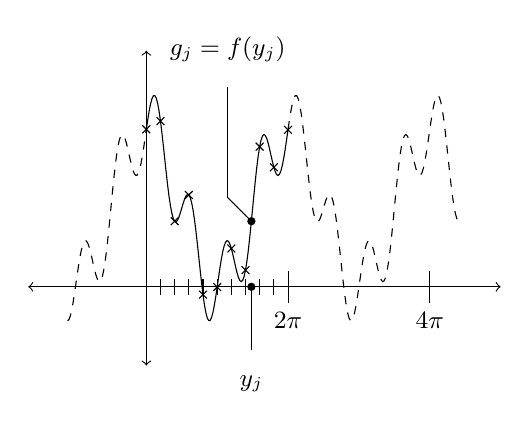
\begin{tikzpicture}
        \draw[<->] (-1.5, 0) -- (4.5, 0);
        \draw[<->] (0, -1) -- (0, 3);
        \draw[-] (1.8, 0.2) -- (1.8, -0.2) node [below] {\small $2\pi$};
        \draw[-] (3.6, 0.2) -- (3.6, -0.2) node [below] {\small $4\pi$};
        \foreach \x in {0.18, 0.36, ..., 1.8} {
          \draw[-] (\x, 0.1) -- (\x, -0.1);
        }

        \fill[black] (1.334, 0) circle (1.5pt);
        \fill[black] (1.334, 0.8334) circle (1.5pt);

        \draw [-] (1.334, 0) -- (1.334, -0.8);
        \draw (1.334, -1.0) node [below] {\small $y_j$};

        \draw [-] (1.334, 0.8334) -- (1.034, 1.1334);
        \draw [-] (1.034, 1.1334) -- (1.034, 2.5334);
        \draw (1.034, 2.7334) node [above] {\small $g_j = f(y_j)$};

        \draw[domain=0:1.8, samples=101, mark=x, mark repeat=10] plot (\x, {0.5*sin(2*pi*4*\x r/1.8) + cos(2*pi*\x r/1.8) + 1});
        \draw[domain=-1.0:0, samples=60, dashed] plot (\x, {0.5*sin(2*pi*4*\x r/1.8) + cos(2*pi*\x r/1.8) + 1});
        \draw[domain=1.8:4.0, samples=120, dashed] plot (\x, {0.5*sin(2*pi*4*\x r/1.8) + cos(2*pi*\x r/1.8) + 1});
      \end{tikzpicture} \\
      {\footnotesize \emph{Interpolating $g_j$ from equispaced samples of $f$.}}
    \end{center}
  }

  \headerbox{Fast Multipole Method}{name = fmm, column = 1, below = band-interp}{

    In our NUFFT algorithm, the kernel $\Phi(y, x) = (y - x)^{-1}$ is
    evaluated using a 1D FMM. The FMM algorithm is simpler and
    more efficient in the 1D case. 

    \vspace{0.293cm}

    % \begin{align*}
    %   \Phi(y, x) = \sum_{m=0}^\infty a(x, x_*) R_m(y - x_*)
    % \end{align*}

    % \begin{align*}
    %   \Phi(y, x) = \sum_{m=0}^\infty b(x, x_*) S_m(y - x_*)
    % \end{align*}

    \begin{center}
      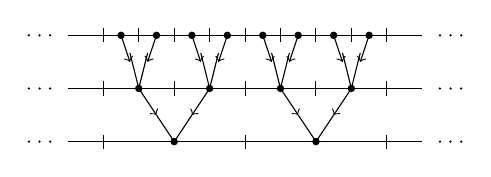
\begin{tikzpicture}[scale = 0.9]
        \foreach \y in {0.75, 0.0, -0.75} {
          \fill[black] (-0.75, \y) circle (0.5pt);
          \fill[black] (-0.9, \y) circle (0.5pt);
          \fill[black] (-1.05, \y) circle (0.5pt);

          \draw [-] (-0.5, \y) -- (4.5, \y);

          \fill[black] (4.75, \y) circle (0.5pt);
          \fill[black] (4.9, \y) circle (0.5pt);
          \fill[black] (5.05, \y) circle (0.5pt);
        }

        \foreach \y in {0.75} {
          \foreach \x in {0.25, 1.25, ..., 3.25} {
            \draw [->] (\x, \y) -- ({\x + 0.125}, {\y / 2});
            \draw [-] ({\x + 0.125}, 0.5) -- ({\x + 0.25}, 0.0);
          }
          \foreach \x in {0.75, 1.75, ..., 3.75} {
            \draw [->] (\x, \y) -- ({\x - 0.125}, {\y / 2});
            \draw [-] ({\x - 0.125}, 0.5) -- ({\x - 0.25}, 0.0);
          }
          \foreach \x in {0.25, 0.75, ..., 3.75} {
            \fill[black] (\x, \y) circle (1.5pt);
          }
          \foreach \x in {0.0, 0.5, ..., 4.0} {
            \draw [-] (\x, {\y + 0.1}) -- (\x, {\y - 0.1});
          }

          \foreach \x in {0.5, 2.5} {
            \draw [->] (\x, 0.0) -- ({\x + 0.25}, {-\y / 2});
            \draw [-] ({\x + 0.25}, {-\y / 2}) -- ({\x + 0.5}, {-\y});
          }
          \foreach \x in {1.5, 3.5} {
            \draw [->] (\x, 0.0) -- ({\x - 0.25}, {-\y / 2});
            \draw [-] ({\x - 0.25}, {-\y / 2}) -- ({\x - 0.5}, {-\y});
          }

          \foreach \x in {1.0, 3.0} {
            \fill[black] (\x, {-\y}) circle (1.5pt);
          }
          \foreach \x in {0.0, 2.0, 4.0} {
            \draw [-] (\x, {-\y + 0.1}) -- (\x, {-\y - 0.1});
          }
        }

        \foreach \x in {0.5, 1.5, ..., 3.5} {
          \fill[black] (\x, 0.0) circle (1.5pt);
        }

        \foreach \x in {0.0, 1.0, 2.0, 3.0, 4.0} {
          \draw [-] (\x, 0.1) -- (\x, -0.1);
        }

        
      \end{tikzpicture} \\
      \vspace{0.1cm}
      {\footnotesize \emph{The upward pass of the FMM.}}
    \end{center}

    \vspace{0.2cm}

    The translation kernels for $\Phi$ that are used in the FMM
    have a structure that can be efficiently computed.

    \vspace{0.2cm}

    \begin{center}
      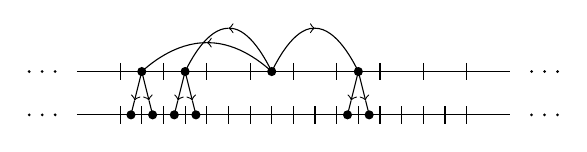
\begin{tikzpicture}[scale = 1.1]
        \foreach \y in {0.5, 0.0} {
          \fill[black] (-0.75, \y) circle (0.5pt);
          \fill[black] (-0.9, \y) circle (0.5pt);
          \fill[black] (-1.05, \y) circle (0.5pt);
          \draw [-] (-0.5, \y) -- (4.5, \y);
          \fill[black] (4.75, \y) circle (0.5pt);
          \fill[black] (4.9, \y) circle (0.5pt);
          \fill[black] (5.05, \y) circle (0.5pt);
        }
        
        \foreach \x in {0.0, 0.5, ..., 4.0} {
          \draw [-] (\x, 0.6) -- (\x, 0.4);
        }

        \foreach \x in {0.25, 0.75, 1.75, 2.75} {
          \fill[black] (\x, 0.5) circle (1.5pt);
        }

        \foreach \x in {0.25, 0.75, 2.75} {
          \draw [->] (\x, 0.5) -- ({\x - 0.125*2/3}, {0.5 - 0.5*2/3});
          \draw [-] ({\x - 0.125*2/3}, {0.5 - 0.5*2/3}) -- ({\x - 0.125}, 0.0);
          \draw [->] (\x, 0.5) -- ({\x + 0.125*2/3}, {0.5 - 0.5*2/3});
          \draw [-] ({\x + 0.125*2/3}, {0.5 - 0.5*2/3}) -- ({\x + 0.125}, 0.0);
        }

        \foreach \x in {0.0, 0.25, ..., 4.0} {
          \draw [-] (\x, 0.1) -- (\x, -0.1);
        }

        \foreach \x in {0.125, 0.375, 0.625, 0.875, 2.625, 2.875} {
          \fill [black] (\x, 0.0) circle (1.5pt);
        }

        \foreach \x in {0.25, 0.75, 2.75} {
          \draw [->] (1.75, 0.5) parabola bend ({(1.75 + \x)/2}, {0.5/abs(\x - 1.75) + 0.5}) ({(1.75 + \x)/2}, {0.5/abs(\x - 1.75) + 0.5});
          \draw [-] ({(1.75 + \x)/2}, {0.5/abs(\x - 1.75) + 0.5}) parabola (\x, 0.5);
        }
      \end{tikzpicture} \\
      \vspace{0.1cm}
      \emph{\footnotesize A step in the downward pass of the FMM.}
    \end{center}
  }

  \headerbox{Periodic Summation}{name = per-sum, column = 2, row = 0}{

    \begin{center}
      \vspace{0.2cm}
      \begin{tikzpicture}[scale = 0.9]
        \draw[-] (-0.6,0) -- (2.6, 0);
        \draw[-] (0, 0.1) -- (0, -0.1);
        \draw (0, -0.3) node[below] {\small $0$};
        \fill[black] (1, 0) circle (1pt);
        \draw[dashed] (1, 0) -- (1, -1);
        \draw (1, -1.2) node[below] {\small $x_* = \pi$};
        \draw[-] (2, 0.1) -- (2, -0.1);
        \draw (2, -0.3) node[below] {\small $2\pi$};
        
        \fill[black] (-0.85, 0) circle (0.5pt);
        \fill[black] (-1.0, 0) circle (0.5pt);
        \fill[black] (-1.15, 0) circle (0.5pt);

        \fill[black] (2.85, 0) circle (0.5pt);
        \fill[black] (3.0, 0) circle (0.5pt);
        \fill[black] (3.15, 0) circle (0.5pt);

        \draw[->] (-1.4, 0) -- (-2.25, 0);
        \draw[-] (-2, 0.1) -- (-2, -0.1);
        \draw (-2, -0.3) node[below] {\small $-2\pi n$};

        \draw[->] (3.4, 0) -- (4.25, 0);
        \draw[-] (4, 0.1) -- (4, -0.1);
        \draw (4, -0.3) node[below] {\small $2\pi (n + 1)$};

        \draw[dashed] (1, 1.1) -- (3.7, 1.1);
        \draw[-] (1, 1.2) -- (1, 1.0);
        \draw[-] (2.7, 1.4) -- (2.7, 1.0);
        \draw (2.7, 1.6) node [above] {\small $r + \pi$};
        \draw[-] (3.32, 1.2) -- (3.32, 0.8);
        \draw (3.32, 0.6) node[below] {\small $R + \pi$};
      \end{tikzpicture} \\
      {\footnotesize \emph{The intervals $(x_* - r, x_* + r)$ and
          $(x_* - R, x_* + R)$ and their bounding box.}}
      \vspace{0.2cm}
    \end{center}

    We use a simplified version of the periodic summation method
    presented in~\cite{gumerov-periodic-sums}. The method is used to evaluate the function:
    \begin{align*}
      \phi(y) &= \sum_{l=-\infty}^\infty \sum_{k=0}^{2K-1} f_k \Phi(y, x_k + 2 \pi l) \\
      &\overset{\Delta}{=} \phinear(y) + \phifar(y)
    \end{align*}
    where $\phinear$ consists of the terms of the outer summation
    where $l \in [-n, n] \subseteq \mathbb{N}$ and $\phifar$ involves
    the terms where $l \notin [-n, n]$. \\

    For $\set{y_j} \subseteq [0, 2\pi)$ (the evaluation domain), the
    algorithm computes $\phi(y_j)$ as follows: 
    { \small
      \begin{enumerate}
      \item \textbf{Compute $\phinear$ using the FMM.} Select a pair
        of intervals centered at $x_* = \pi$. Evaluate $\phinear$ at
        each point $y_j$ and at a periodically offset check point
        $\tilde{y}_j = y_j - 2\pi l$.
      \item \textbf{Evaluate $\phifar$ using least squares collocation.}
        Compute $\phifar$ approximately via an expansion in the FMM's
        local basis functions in the evaluation domain.
      \item \textbf{Compute $\phi = \phinear + \phifar$ by summing.}
        % \item Compute the coefficients $\bold{c}$ of $\phifar$ from:
        %   \begin{align*}
        %     -\bold{R} \bold{c} = \boldsymbol{\phi}_{\operatorname{near}}
        %   \end{align*}
      \end{enumerate}
    }

    % \begin{align*}
    %   \mathcal{N} = [-n, n] \subseteq \mathbb{Z}
    % \end{align*}


    % \begin{align*}
    %   \phinear(y) &= \sum_{l \in \mathcal{N}} \sum_{k=0}^{2K-1} f_k \Phi(y, x_k + 2 \pi l) \\
    %   \phifar(y) &= \sum_{l \notin \mathcal{N}} \sum_{k=0}^{2K-1} f_k \Phi(y, x_k + 2 \pi l)
    % \end{align*}

    \begin{center} 
      \vspace{0.2cm}
      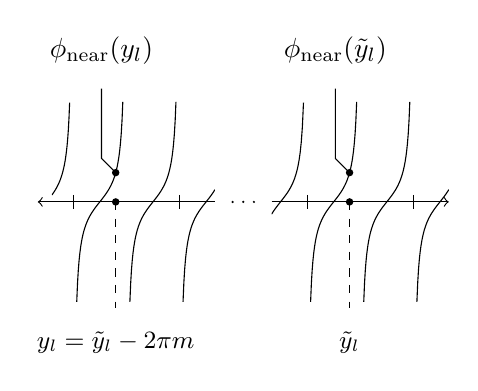
\begin{tikzpicture}[scale = 0.9]
        \draw [<-] (-0.5, 0) -- (2.0, 0);
        % \draw [dashed] (2.0, 0) -- (3.0, 0);
        \fill[black] (2.25, 0) circle (0.5pt);
        \fill[black] (2.4, 0) circle (0.5pt);
        \fill[black] (2.55, 0) circle (0.5pt);
        \draw [->] (2.8, 0) -- (5.3, 0);
        \draw [-] (3.3, 0.1) -- (3.3, -0.1);
        % \draw (3.3, -0.3) node [below] {\small $2\pi n$};
        \draw [-] (4.8, 0.1) -- (4.8, -0.1);
        % \draw (4.8, -0.3) node [below] {\small $2\pi (n+1)$};

        \fill[black] (0.6, 0.) circle (1.5pt);
        \draw [dashed] (0.6, 0) -- (0.6, -1.5);
        \draw (0.6, -1.7) node [below] {\small $y_l = \tilde{y}_l - 2\pi m$};

        \fill[black] (0.6, 0.4129) circle (1.5pt);
        \draw [-] (0.6, 0.4129) -- (0.4, 0.6129) -- (0.4, 1.6);
        \draw (0.4, 1.8) node [above] {$\phinear(y_l)$};

        \fill[black] (3.9, 0) circle (1.5pt);
        \draw [dashed] (3.9, 0) -- (3.9, -1.5);
        \draw (3.9, -1.7) node [below] {\small $\tilde{y}_l$};

        \fill[black] (3.9, 0.4129) circle (1.5pt);
        \draw [-] (3.9, 0.4129) -- (3.7, 0.6129) -- (3.7, 1.6);
        \draw (3.7, 1.8) node [above] {$\phinear(\tilde{y}_l)$};

        \draw [-] (0, 0.1) -- (0, -0.1);
        % \draw (0.0, -0.3) node [below] {\small $0$};
        \draw [-] (1.5, 0.1) -- (1.5, -0.1);
        % \draw (1.5, -0.3) node [below] {\small $2\pi$};

        \begin{scope}
          \clip (0.0, 1.5) rectangle (1.5, -1.5);
          \draw[domain=0.05:0.7, samples=60] plot (\x, {-0.3*cot(2 * pi * \x r / 1.5)});
          \draw[domain=0.8:1.45, samples=60] plot (\x, {-0.3*cot(2 * pi * \x r / 1.5)});
        \end{scope}
        \begin{scope}
          \clip (-0.3, 1.5) rectangle (0.0, -1.5);
          \draw[domain=-0.3:-0.05, samples=30] plot (\x, {-0.3*cot(2 * pi * \x r / 1.5)});
        \end{scope}
        \begin{scope}
          \clip (1.5, 1.5) rectangle (2.0, -1.5);
          \draw[domain=1.55:2.0, samples=40] plot (\x, {-0.3*cot(2 * pi * \x r / 1.5)});
        \end{scope}

        \begin{scope}[shift = {(3.3, 0)}]
          \begin{scope}
            \clip (0.0, 1.5) rectangle (1.5, -1.5);
            \draw[domain=0.05:0.7, samples=60] plot (\x, {-0.3*cot(2 * pi * \x r / 1.5)});
            \draw[domain=0.8:1.45, samples=60] plot (\x, {-0.3*cot(2 * pi * \x r / 1.5)});
          \end{scope}
          \begin{scope}
            \clip (-0.5, 1.5) rectangle (0.0, -1.5);
            \draw[domain=-0.5:-0.05, samples=30] plot (\x, {-0.3*cot(2 * pi * \x r / 1.5)});
          \end{scope}
          \begin{scope}
            \clip (1.5, 1.5) rectangle (2.0, -1.5);
            \draw[domain=1.55:2.0, samples=40] plot (\x, {-0.3*cot(2 * pi * \x r / 1.5)});
          \end{scope}
        \end{scope}

      \end{tikzpicture} \\
      \vspace{0.128cm}
      {\footnotesize \emph{The periodically offset check points used
          in computing the coefficients of $\phifar$.}}
      \vspace{0.08cm}
    \end{center}

    % \begin{itemize}
    % \item $\parens{\bold{R}}_{i,m} \equiv \Delta_{2 \pi l}[R_m](y_i - x_*)$,
    % \item $\parens{\bold{c}}_m \equiv c_m$,
    % \item $\parens{\boldsymbol{\phi}_{\operatorname{near}}}_i \equiv \Delta_{2\pi l}[\phinear](y_i)$,
    % \item $\parens{\boldsymbol{\epsilon}^{(p)}}_i \equiv \Delta_{2\pi l}[\epsilon^{(p)}](y_i)$.
    % \end{itemize}

    % \begin{align*}
    %   \bold{c} \approx -\bold{R}^\dagger \parens{\boldsymbol{\phi} + \boldsymbol{\epsilon}^{(p)}}
    % \end{align*}
  }

  \headerbox{Preliminary Results}{name = prelim-results, column = 3, row = 0}{

    Our prototype was written in Julia and compared against direct
    interpolation to demonstrate the viability of the algorithm. In
    all of our numerical experiments, an FMM was used that ensured
    a high degree of accuracy.

    \begin{center}
      \vspace{0.15cm}
      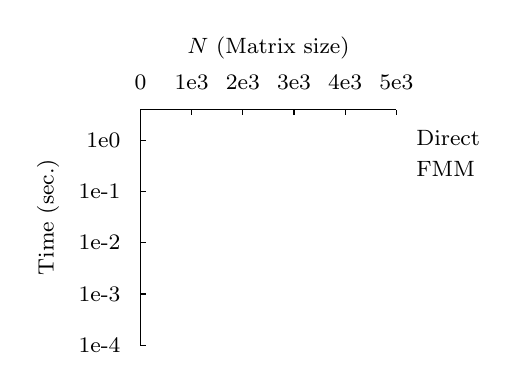
\begin{tikzpicture}[scale = 0.65]
        \draw [-] (0, 0.6) -- (0, -4.0);
        \draw [-] (0.0, 0.6) -- (5.0, 0.6);
        \draw (0.0, 0.8) node [above] {\footnotesize 0};
        \draw (1.0, 0.8) node [above] {\footnotesize 1e3};
        \draw (2.0, 0.8) node [above] {\footnotesize 2e3};
        \draw (3.0, 0.8) node [above] {\footnotesize 3e3};
        \draw (4.0, 0.8) node [above] {\footnotesize 4e3};
        \draw (5.0, 0.8) node [above] {\footnotesize 5e3};
        \draw (2.5, 1.4) node [above] {\footnotesize $N$ (Matrix size)};
        \foreach \x in {1.0, 2.0, ..., 5.0} {
          \draw [-] (\x, 0.6) -- (\x, 0.5);
        }
        \foreach \y in {0.0, -1.0, ..., -4.0} {
          \draw [-] (0, \y) -- (0.1, \y);
        }
        \draw (-0.2, 0.0) node [left] {\footnotesize 1e0};
        \draw (-0.2, -1.0) node [left] {\footnotesize 1e-1};
        \draw (-0.2, -2.0) node [left] {\footnotesize 1e-2};
        \draw (-0.2, -3.0) node [left] {\footnotesize 1e-3};
        \draw (-0.2, -4.0) node [left] {\footnotesize 1e-4};
        \draw (-1.4, -1.5) node [left] {\footnotesize \rotatebox{90}{Time (sec.)}};
        \begin{scope}
          \clip (0.0, 0.6) rectangle (5.0, -4.0);
          \draw plot[smooth] file {directtimes.txt};
        \end{scope}
        \draw plot[smooth] file {fmmtimes.txt};
        \draw (5.2, 0.05) node [right] {\footnotesize Direct};
        \draw (5.2, -0.55) node [right] {\footnotesize FMM};
      \end{tikzpicture} \\
      {\footnotesize \emph{Direct evaluation of $\phi$ vs. FMM evaluation.}}
      \vspace{0.14cm}
    \end{center}

    \begin{center}
      \vspace{0.14cm}
      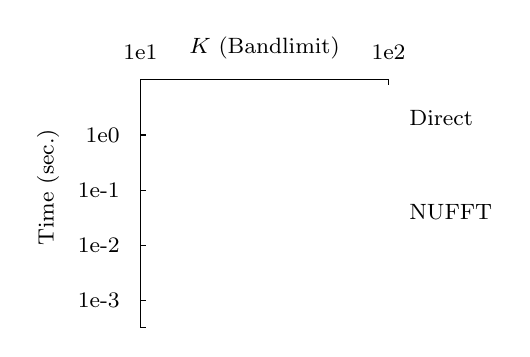
\begin{tikzpicture}[scale = 0.7]
        \draw [-] (0.5, 1.0) -- (0.5, -3.5);
        \draw [-] (0.5, 1.0) -- (5.0, 1.0);
        \draw [-] (5.0, 1.0) -- (5.0, 0.9);
        \foreach \y in {0.0, -1.0, ..., -3.0} {
          \draw [-] (0.5, \y) -- (0.6, \y);
        }
        \draw [-] (0.5, -3.5) -- (0.6, -3.5);
        \draw plot[smooth] file {gtavg.txt};
        \draw plot[smooth] file {persumavg.txt};
        \draw (2.75, 1.2) node [above] {\footnotesize $K$ (Bandlimit)};
        \draw (-0.8, -0.95) node [left] {\footnotesize \rotatebox{90}{Time (sec.)}};
        \draw (0.5, 1.2) node [above] {\footnotesize 1e1};
        \draw (5.0, 1.2) node [above] {\footnotesize 1e2};
        \draw (0.3, 0.0) node [left] {\footnotesize 1e0};
        \draw (0.3, -1.0) node [left] {\footnotesize 1e-1};
        \draw (0.3, -2.0) node [left] {\footnotesize 1e-2};
        \draw (0.3, -3.0) node [left] {\footnotesize 1e-3};
        \draw (5.2, 0.3) node [right] {\footnotesize Direct};
        \draw (5.2, -1.4) node [right] {\footnotesize NUFFT};
      \end{tikzpicture} \\
      {\footnotesize \emph{Computation of $\mathcal{P}(\bold{f})$: direct vs. NUFFT.}}
      \vspace{0.124cm}
    \end{center}
  }

  \headerbox{Future Work}{name = future-work, column = 3, below = prelim-results}{

    The approach used for computing
    $\mathcal{P} \circ \mathcal{F}^{-1}$ will be applied to
    $\mathcal{F} \circ \mathcal{P}^{-1}$. A careful error analysis
    involving checkpoints will be carried out; different distributions
    of checkpoints will be explored. The implementation can be
    optimized significantly; the algorithm itself can be improved by
    making use of an adaptive FMM.

  }

  \headerbox{References}{name = references, column = 3, below = future-work}{
    {
      \small
      \bibliographystyle{plain}
      \renewcommand{\section}[2]{\vskip 0.05em}
      \begin{thebibliography}{1}
      \bibitem{gumerov-periodic-sums} Nail A. Gumerov and Ramani Duraiswami. A method to compute periodic sums, 2014. \emph{J. Comput. Phys.}, 272:307-326, 2014.
      \bibitem{dutt-rokhlin-ii} A. Dutt and V. Rokhlin. Fast fourier transforms for nonequispaced data, II. \emph{Appl. Comput. Harmon. Anal.}, 2:85-100, 1995.
      \end{thebibliography}
    }
  }
  
\end{poster}

\end{document}